\documentclass[11pt]{article}
\usepackage{graphicx}
\graphicspath{ {./pictures/} }

\usepackage[hoptionsi]{subcaption}

%%%%%%%%%%%%%%%%%%%%%%%%%%%%%%%%%%%%%%%%%
% Lachaise Assignment
% Structure Specification File
% Version 1.0 (26/6/2018)
%
% This template originates from:
% http://www.LaTeXTemplates.com
%
% Authors:
% Marion Lachaise & François Févotte
% Vel (vel@LaTeXTemplates.com)
%
% License:
% CC BY-NC-SA 3.0 (http://creativecommons.org/licenses/by-nc-sa/3.0/)
% 
%%%%%%%%%%%%%%%%%%%%%%%%%%%%%%%%%%%%%%%%%

%----------------------------------------------------------------------------------------
%	PACKAGES AND OTHER DOCUMENT CONFIGURATIONS
%----------------------------------------------------------------------------------------

\usepackage{amsmath,amsfonts,stmaryrd,amssymb} % Math packages

\usepackage{enumerate} % Custom item numbers for enumerations

\usepackage[ruled]{algorithm2e} % Algorithms

\usepackage[framemethod=tikz]{mdframed} % Allows defining custom boxed/framed environments

\usepackage{listings} % File listings, with syntax highlighting
\lstset{
	basicstyle=\ttfamily, % Typeset listings in monospace font
}

%----------------------------------------------------------------------------------------
%	DOCUMENT MARGINS
%----------------------------------------------------------------------------------------

\usepackage{geometry} % Required for adjusting page dimensions and margins

\geometry{
	paper=a4paper, % Paper size, change to letterpaper for US letter size
	top=2.5cm, % Top margin
	bottom=3cm, % Bottom margin
	left=2.5cm, % Left margin
	right=2.5cm, % Right margin
	headheight=14pt, % Header height
	footskip=1.5cm, % Space from the bottom margin to the baseline of the footer
	headsep=1.2cm, % Space from the top margin to the baseline of the header
	%showframe, % Uncomment to show how the type block is set on the page
}

%----------------------------------------------------------------------------------------
%	FONTS
%----------------------------------------------------------------------------------------

\usepackage[utf8]{inputenc} % Required for inputting international characters
\usepackage[T1]{fontenc} % Output font encoding for international characters

\usepackage{XCharter} % Use the XCharter fonts

%----------------------------------------------------------------------------------------
%	COMMAND LINE ENVIRONMENT
%----------------------------------------------------------------------------------------

% Usage:
% \begin{commandline}
%	\begin{verbatim}
%		$ ls
%		
%		Applications	Desktop	...
%	\end{verbatim}
% \end{commandline}

\mdfdefinestyle{commandline}{
	leftmargin=10pt,
	rightmargin=10pt,
	innerleftmargin=15pt,
	middlelinecolor=black!50!white,
	middlelinewidth=2pt,
	frametitlerule=false,
	backgroundcolor=black!5!white,
	frametitle={Command Line},
	frametitlefont={\normalfont\sffamily\color{white}\hspace{-1em}},
	frametitlebackgroundcolor=black!50!white,
	nobreak,
}

% Define a custom environment for command-line snapshots
\newenvironment{commandline}{
	\medskip
	\begin{mdframed}[style=commandline]
}{
	\end{mdframed}
	\medskip
}

%----------------------------------------------------------------------------------------
%	FILE CONTENTS ENVIRONMENT
%----------------------------------------------------------------------------------------

% Usage:
% \begin{file}[optional filename, defaults to "File"]
%	File contents, for example, with a listings environment
% \end{file}

\mdfdefinestyle{file}{
	innertopmargin=1.6\baselineskip,
	innerbottommargin=0.8\baselineskip,
	topline=false, bottomline=false,
	leftline=false, rightline=false,
	leftmargin=2cm,
	rightmargin=2cm,
	singleextra={%
		\draw[fill=black!10!white](P)++(0,-1.2em)rectangle(P-|O);
		\node[anchor=north west]
		at(P-|O){\ttfamily\mdfilename};
		%
		\def\l{3em}
		\draw(O-|P)++(-\l,0)--++(\l,\l)--(P)--(P-|O)--(O)--cycle;
		\draw(O-|P)++(-\l,0)--++(0,\l)--++(\l,0);
	},
	nobreak,
}

% Define a custom environment for file contents
\newenvironment{file}[1][File]{ % Set the default filename to "File"
	\medskip
	\newcommand{\mdfilename}{#1}
	\begin{mdframed}[style=file]
}{
	\end{mdframed}
	\medskip
}

%----------------------------------------------------------------------------------------
%	NUMBERED QUESTIONS ENVIRONMENT
%----------------------------------------------------------------------------------------

% Usage:
% \begin{question}[optional title]
%	Question contents
% \end{question}

\mdfdefinestyle{question}{
	innertopmargin=1.2\baselineskip,
	innerbottommargin=0.8\baselineskip,
	roundcorner=5pt,
	nobreak,
	singleextra={%
		\draw(P-|O)node[xshift=1em,anchor=west,fill=white,draw,rounded corners=5pt]{%
		Question \theQuestion\questionTitle};
	},
}

\newcounter{Question} % Stores the current question number that gets iterated with each new question

% Define a custom environment for numbered questions
\newenvironment{question}[1][\unskip]{
	\bigskip
	\stepcounter{Question}
	\newcommand{\questionTitle}{~#1}
	\begin{mdframed}[style=question]
}{
	\end{mdframed}
	\medskip
}

%----------------------------------------------------------------------------------------
%	WARNING TEXT ENVIRONMENT
%----------------------------------------------------------------------------------------

% Usage:
% \begin{warn}[optional title, defaults to "Warning:"]
%	Contents
% \end{warn}

\mdfdefinestyle{warning}{
	topline=false, bottomline=false,
	leftline=false, rightline=false,
	nobreak,
	singleextra={%
		\draw(P-|O)++(-0.5em,0)node(tmp1){};
		\draw(P-|O)++(0.5em,0)node(tmp2){};
		\fill[black,rotate around={45:(P-|O)}](tmp1)rectangle(tmp2);
		\node at(P-|O){\color{white}\scriptsize\bf !};
		\draw[very thick](P-|O)++(0,-1em)--(O);%--(O-|P);
	}
}

% Define a custom environment for warning text
\newenvironment{warn}[1][Warning:]{ % Set the default warning to "Warning:"
	\medskip
	\begin{mdframed}[style=warning]
		\noindent{\textbf{#1}}
}{
	\end{mdframed}
}

%----------------------------------------------------------------------------------------
%	INFORMATION ENVIRONMENT
%----------------------------------------------------------------------------------------

% Usage:
% \begin{info}[optional title, defaults to "Info:"]
% 	contents
% 	\end{info}

\mdfdefinestyle{info}{%
	topline=false, bottomline=false,
	leftline=false, rightline=false,
	nobreak,
	singleextra={%
		\fill[black](P-|O)circle[radius=0.4em];
		\node at(P-|O){\color{white}\scriptsize\bf i};
		\draw[very thick](P-|O)++(0,-0.8em)--(O);%--(O-|P);
	}
}

% Define a custom environment for information
\newenvironment{info}[1][Info:]{ % Set the default title to "Info:"
	\medskip
	\begin{mdframed}[style=info]
		\noindent{\textbf{#1}}
}{
	\end{mdframed}
}
 % Include the file specifying the document structure and custom commands

%----------------------------------------------------------------------------------------
%	ASSIGNMENT INFORMATION
%----------------------------------------------------------------------------------------

\title{Dynamic Distributed Decision Making \\Project 1 \\MIE567} % Title of the assignment

\author{\texttt{Hao Tan 999735728}\\ \texttt{Xiali Wu 999011322} \\ \texttt{David Molina 1005615318}} % Author name and email address

\date{University of Toronto --- \today} % University, school and/or department name(s) and a date

%----------------------------------------------------------------------------------------

\begin{document}

\maketitle

\section{Modelling}
\textbf{First, you are tasked with modelling the Gridworld domain
above as a Markov decision process. Then, you are asked to provide a complete
programming description of the problem that will be used to solve it
computationally.}
\\

% 1---------------------------------------------------------------
\noindent
\textbf{1}
\noindent
\textbf{Explain how you would model this navigation problem as a Markov
decision process. In particular:}
\\

% 1A---------------------------------------------------------------
\noindent
\textbf{a)}
\noindent
\textbf{Why is this problem an MDP? }
\\

\noindent
This problem can be described as an MDP because it can be modeled in terms of
components such as a reward function, actions, transition probability, states,
time steps and discount factor. Additionally, this problem is an infinite
horizon MDP since we can take unlimited amounts of steps between cells, and
possibly re-visit the same cell. In this case, unlimited amount of steps can
potentially happen to maximize rewards; therefore, a discount factor is included
for future rewards.
\\

\noindent
Furthermore, based on the definition of Markovian property, a stochastic process
has the Markov property if the conditional probability distribution of future
states of the process (conditional on both past and present states) depends only
upon the present state, not on the sequence of events that preceded it (ie.
P[St+1 | St] = P[St+1 | S1, S2 ... St]). In the given problem description, the
agent can only move one cell per action, while the next cell is only dependent
on the current cell. In other words, the next cell is not dependent on previous
cells before the current cell.
\\

% 1B---------------------------------------------------------------
\noindent
\textbf{b)}
\noindent
\textbf{What are suitable state and action spaces for this problem? Are
these the only possible choices? Why or why not?}
\\

\noindent
The states can be represented as the coordinates of the grid world (i,j), where i=
0,..,4, and j=0,...,4, as seen in the following.

\begin{equation}
\text { states }=\left[\begin{array}{lllll}
{(0,0)} & {(0,1)} & {(0,2)} & {(0,3)} & {(0,4)} \\
{(1,0)} & {(1,1)} & {(1,2)} & {(1,3)} & {(1,4)} \\
{(2,0)} & {(2,1)} & {(2,2)} & {(2,3)} & {(2,4)} \\
{(3,0)} & {(3,1)} & {(3,2)} & {(3,3)} & {(3,4)} \\
{(4,0)} & {(4,1)} & {(4,2)} & {(4,3)} & {(4,4)}
\end{array}\right]
\end{equation}


\noindent
The available set of actions are North, East, West, South, which can be implemented
using the addition and subtraction of grid world coordinates. For example, the following
shows the possible actions where (-1, 0) means North, (0,1) means East, (1,0) means South,
and (0,-1) means West.

\begin{equation}
\text { actions }=[(-1,0),(0,1),(1,0),(0,-1)]
\end{equation}

\noindent
There are other alternatives for the representation of this problem, for
example, each cells can be represented with a number from 1 to 25 and actions
can be represented as letters A = {N, E, W, S} or {up, right, down, left}. These
type of representations are tidieous to implement. For example, using continuous
numbers to represent states would be difficult to stop the agent from moving
off-grid without excessive \textit{if-statements}. In terms of other possible
actions, one may considerd diagonal actions such as those shown below.

\begin{equation}
\text { diagonal actions }=[(1,1),(-1,1),(1,-1),(-1,-1)]
\end{equation}

\noindent
Diagonal actions require the agent to move two steps per action to arrive at the
intended cell. For example, to move North-West, the agent must move West then
Easy or vice versa. This conflicts with the problem description where the agent
is only allowed to move one cell at a time; therefore, this alternative  not
used in the model. \\


% 1C---------------------------------------------------------------
\noindent
\textbf{c)}
\noindent
\textbf{What is the transition probability matrix P? (You may describe just
the non-zero entries.)}
\\

\noindent
In a transition probability matrix, the sum of each row is equal to one. In the
transition probability matrix presented in the Appendix, the vertical axis along
the left represents the current state, $s$, while the horizontal axis along the
top represents the potential next state, $s'$. Assuming a random policy with
equal probability distribution for all actions, there is a 25\% chance of
arriving at the intended neighbor cell except for the cells along the border of
the grid. For the cells at each of the corners, there are 2 actions each that
would take the agent off grid. In this scenario, the problem description states
that the agent would remain in its current position; therefore, the corner
states have a 50\% chance of transitioning to its own state and 25\% chance of
transitioning to a neighbor state. The same logic can be applied for the other
border states, where there is always a probability of returning to its own state
if an off-grid action is taken. Additionally, there are 2 special states;
namely, State A and B where all actions would take the agent directly to A' and
B', respectively. The transition probability matrix is presented in the
\textbf{Appendix} \\

% 1D---------------------------------------------------------------
\noindent
\textbf{d)}
\noindent
\textbf{Is the reward function provided the only possible one? If so, explain
why. If not, provide an example of a different reward function that would lead
to the same optimal behaviour}
\\

\noindent
The reward function privided is by the problem is shown below. In this case, a
transition from A to A' and B to B' will yield a reward of 10 and 5,
respectively. A transition that would take the agent off grid would result in a
reward of -1 while all other transitions yield a reward of zero. 

\begin{equation}
\text { Reward }={[0,-1,+5,+10]}
\end{equation}

\noindent
Using the state and action representation described in previous questions, an
off grid action is detected when elements within the next state coordinate holds
a value greater or less than the column/row size. For example, the following
show two cases of an agent going off grid. In equation (5), the agent is
originally in state (0,0) and the chosen action is to the left/West (0, -1),
this results in a coordinate (0, -1) that featured an element smaller than the
grid column/row size. Conversely, in equation (6), the agent took an action
going to the right when in state (0, 4) which resulted in the next state, (0,
5), with an element larger than the row/column size. In these cases, the agent
receives a reward of 1.

\noindent
By having a different reward function, the overall optimization problem is different.
As a result, this is the only reward function that leads to optimal
behaviour as described in the problem description. <DOES MULTIPLES OF THE SAME GENERATE THE SAME BEHAVIOUR?>

\begin{equation}
\left[\begin{array}{c}
{0} \\
{0}
\end{array}\right]+\left[\begin{array}{c}
{0} \\
{-1}
\end{array}\right]=\left[\begin{array}{c}
{0} \\
{-1}
\end{array}\right]
\end{equation}

\begin{equation}
\left[\begin{array}{l}
{0} \\
{4}
\end{array}\right]+\left[\begin{array}{l}
{0} \\
{1}
\end{array}\right]=\left[\begin{array}{l}
{0} \\
{5}
\end{array}\right]
\end{equation}
\\

% 1E---------------------------------------------------------------
\noindent
\textbf{e)}
\noindent
\textbf{Derive the discounted Bellman equation for the problem, and simplify
as much as you can. (Hint: to avoid deriving a separate value for each state,
try to find groups of states such that you can write a single expression for V for
them) What do you think is/are the optimal policy/policies for this problem,
and why (you do NOT need to solve the Bellman equations)?}
\\



\noindent
To write the Bellman equations for this problem, we have grouped together states
with similar value functions as represented by the different colors in the figure below.
<STATE THE INTUITION BEHIND THE PRESENTED GROUPING>
\\

\noindent
Since the goal is maximizing reward, optimal policy always looks for A or B to
gain +10 or +5 reward. If the initial state is away from row 0 where A and B are
located, such as row 4, the optimal policy would direct the agent to the
vicinity of A or B. If the initial state is in the vicinity of A and B, there is
a tradeoff between more actions towards A and earning discounted +5 more reward
from A->A’ compared to B->B’.
\\

\begin{figure}[h]
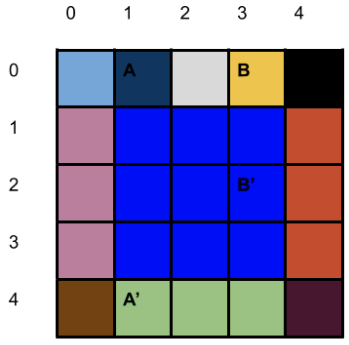
\includegraphics[scale=0.4]{bellman_groups}
\centering
\caption{Groups of Bellman equations}
\end{figure}

\noindent
The following shows the Bellman equation, while equation (8) to (18) shows the different
equations grouped by the colors presented in the above figure.

\begin{equation}
v_{\pi}(s)=\sum_{a} \pi(a | s) \sum_{s^{\prime}, r} p\left(s^{\prime}, r | s, a\right)\left[r+\gamma v_{\pi}\left(s^{\prime}\right)\right]
\end{equation}


% 1E BELLMAN EQUATIONS -----------------------------------------------------
\noindent
The following represents the value function for state (0, 0)

\begin{equation}
\begin{array}{c}
{P([0,-1] |(i, j))(-1+\gamma v(i, j))+P([-1,0] |(i, j))(-1+\gamma v(i, j))} \\
{+P([0,+1](i, j))(0+\gamma v(i, j+1))+P([+1, 0] |(i, j))(0+\gamma v(i+1, j))} \\
{\quad \text { for } i \in\{0\}, j \in\{0\}}
\end{array}
\end{equation}

\noindent
The following represents the value function for state (0, 1)

\begin{equation}
\begin{array}{c}
{P([0,-1] |(i, j))(10+\gamma v(i+4, j))+P([-1,0]|(i,j))(10+\gamma v(i+4, j))} \\
{+P([0,+1] |(i, j))(10+\gamma v(i+4, j))+P([+1,0]|(i,j))(10+\gamma v(i+4, j))} \\
{\quad \text { for } i \in\{0\}, j \in\{1\}}
\end{array}
\end{equation}

\noindent
The following represents the value function for state (0, 2)

\begin{equation}
\begin{array}{c}
{P([0,-1] |(i, j))(0+\gamma v(i, j-1))+P([-1,0] |(i, j))(-1+\gamma v(i, j))} \\
{+P([0,+1] |(i, j))(0+\gamma v(i, j+1))+P([+1,0] |(i, j))(0+\gamma v(i+1, j))} \\
{\quad \text { for } i \in\{0\}, j \in\{2\}}
\end{array}
\end{equation}

\noindent
The following represents the value function for state (0, 3)

\begin{equation}
\begin{array}{c}
{P([0,-1] |(i, j))(5+\gamma v(i+2, j))+P([-1,0] |(i, j))(5+\gamma v(i+2, j))} \\
{+P([0,+1] |(i, j))(5+\gamma v(i+2, j))+P([+1,0] |(i, j))(5+\gamma v(i+2, j))} \\
{\quad \text { for } i \in\{0\}, j \in\{3\}}
\end{array}
\end{equation}

\noindent
The following represents the value function for state (0, 4)

\begin{equation}
\begin{array}{c}
{P([0,-1] |(i, j))(0+\gamma v(i, j-1))+P([-1,0] |(i, j))(-1+\gamma v(i, j))} \\
{+P([0,+1] |(i, j))(-1+\gamma v(i, j))+P([+1,0] |(i, j))(0+\gamma v(i+1, j))} \\
{\quad \text { for } i \in\{0\}, j \in\{4\}}
\end{array}
\end{equation}

\noindent
The following represents the value function for state (1,0), (2,0), (3,0).

\begin{equation}
\begin{array}{c}
{P([0,-1] |(i, j))(-1+\gamma v(i, j))+P([-1,0] |(i, j))(0+\gamma v(i-1, j))}\\
{+P([0,+1] |(i, j))(0+\gamma(i, j+1))+P([+1,0] |(i, j))(0+\gamma v(i+1, j))}\\
{\text { for } i \in\{1,2,3\}, j \in\{0\}}
\end{array}
\end{equation}

\noindent
The following represents the value function for state (1,1), (1,2), (1,3),
(2,1),(2,2),(2,3),\\
(3,1),(3,2),(3,3).

\begin{equation}
\begin{array}{c}
{P([0,-1] |(i, j))(0+\gamma v(i, j-1))+P([-1,0] |(i, j))(0+\gamma v(i-1, j))} \\
{+P([0,+1]|(i, j))( 0+\gamma v(i, j+1))+P([+1,0] |(i, j))(0+\gamma v(i+1, j))} \\
{\quad \text { for } i \in\{1,2,3\}, j \in\{1,2,3\}}
\end{array}
\end{equation}

\noindent
The following represents the value function for state (1,4),(2,4),(3,4).

\begin{equation}
\begin{array}{c}
{P([0,-1]|(i, j))(0+\gamma v(i, j-1))+P([-1,0] |(i, j))(0+\gamma v(i-1, j))} \\
{+P([0,+1]|(i, j))(-1+\gamma v(i, j))+P([+1,0] |(i, j))(0+\gamma v(i+1, j))} \\
{ \text { for } i \in\{1,2,3\}, j \in\{4\}}
\end{array}
\end{equation}

\noindent
The following represents the value function for state (4,0).

\begin{equation}
\begin{array}{c}
{P([0,-1]|(i, j))(-1+\gamma v(i, j))+P([-1,0]|(i, j))(0+\gamma v(i-1, j))} \\
{+P([0,+1]|(i, j))(0+\gamma v(i, j+1))+P([+1,0]|(i, j)(-1+\gamma v(i, j))} \\
{\quad \text{for } i \in\{4\}, j \in\{0\}}
\end{array}
\end{equation}

\noindent
The following represents the value function for state (4,1), (4,2), (4,3).

\begin{equation}
\begin{array}{c}
{P([0,-1] |(i,j))(0+\gamma v(i, j-1))+P([-1,0] |(i, j))(0+\gamma v(i-1, j))} \\
{+P([0,+1] |(i, j))(0+\gamma v(i, j+1))+P([+1,0] |(i, j))(-1+\gamma v(i, j))}\\
{\quad \text { for } i \in\{4\}, j \in\{1,2,3\}}
\end{array}\\
\end{equation}

\noindent
The following represents the value function for state (4,4).

\begin{equation}
\begin{array}{c}
{P([0,-1] |(i, j))(0+\gamma v(i, j-1))+P([-1,0]|(i, j))(0+\gamma v(i-1, j))} \\
{+P([0,+1]|(i, j))(1+\gamma v(i, j))+P([+1,0]|(i,j))(-1+\gamma v(i, j))} \\
{\quad \text { for } i \in\{4\}, j \in\{4\}}
\end{array}
\end{equation}


% 2---------------------------------------------------------------
\noindent
\textbf{2}
\noindent
\textbf{Now, in a Python file called Gridworld.py, create a class that replicates
the behaviour of the MDP you formulated in the previous question. Your class
should contain four functions: one to return the initial state of the MDP, one to
return a view of all possible states, and two to return, respectively, the reward and
probability of a transition (s; a; s') from state s to state s' when taking action a.}
\\

\lstset{language=Python}
\lstset{frame=lines}
\lstset{caption={Returns a random initial state}}
\lstset{label={lst:code_direct}}
\lstset{basicstyle=\footnotesize}
\begin{lstlisting}
    def initial_state(self):
        # randomly generate an initial state
        i = random.randint(0, len(self.states)-1)
        rand_state = self.states[i]
        return rand_state
\end{lstlisting}

\lstset{caption={Returns a view of all possile states}}
\lstset{label={lst:code_direct}}
\lstset{basicstyle=\footnotesize}
\begin{lstlisting}
    def possible_states(self):
        # return the possible states
        return self.states
\end{lstlisting}

\lstset{caption={Returns a reward given current position and action }}
\lstset{label={lst:code_direct}}
\lstset{basicstyle=\footnotesize}
\begin{lstlisting}
    def reward(self, current_pos, action):
        # take action in current pos
        self.new_pos = np.array(current_pos) + np.array(action)
        # normally, reward = 0
        reward = 0
        # if new pos results in off the grid, return reward -1
        if -1 in self.new_pos or self.size in self.new_pos:
            reward = -1
        # if in state A, transition to state A'
        if current_pos == [0, 1]:
            reward = 10
        # if in state B, transition to state B'
        if current_pos == [0, 3]:
            reward = 5
        return reward
\end{lstlisting}

\lstset{caption={Returns the next state, $s'$, given $a$ in state $s$}}
\lstset{label={lst:code_direct}}
\lstset{basicstyle=\footnotesize}
\begin{lstlisting}
    def p_transition(self, current_pos, action):
        self.new_pos = np.array(current_pos) + np.array(action)
        # if taking an action crosses the border = agent stays in same position
        if -1 in self.new_pos or self.size in self.new_pos: 
            self.new_pos = current_pos
        # if in state A, transition to state A'
        if current_pos == [0, 1]:
            self.new_pos = [4, 1]
        # if in state B, transition to state B'
        if current_pos == [0, 3]:
            self.new_pos = [2, 3]
        return self.new_pos
\end{lstlisting}


% POLICY EVALUATION---------------------------------------------------------------
\newpage
\section{Policy Evaluation}
\textbf{Now, suppose the agent selects all four actions with equal probability. Use your
answers to questions 1 and 2 to write a python function, in a new file policy
evaluation.py to find the value function for this policy. You may use either an
iterative method or solve the system of equations. Show the value function you
obtained to at least four decimals.}
\\

\noindent
Using an iterative method, the following figure shows the value function
achieved with a policy that features even probability for all actions. From
this, it is seen that state A and B featured the highest values at 7.1243 and
4.7526, respectively, which makese sense as actions from these two states would
yield a return of +10 and +5. The states towards the bottom of the grid featured
a negative value as they are far from the high rewarding states mentioned
previously. Additionally, states (0,0) and (0,2) have different values despite
being both one cell away from state A because state (0,0) has a higher chance of
going off-grid than state (0,2).


\begin{figure}[h]
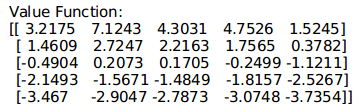
\includegraphics[scale=0.6]{v_evaluation}
\centering
\caption{Value function using policy evaluation}
\end{figure}

\noindent
The following shows a graph of the change in max delta over iterations. From
this, it is seen that the policy evaluation algorithm was able to converge in
roughly 900 iterations with a threshold of $10^{-6}$. \\

\begin{figure}[h]
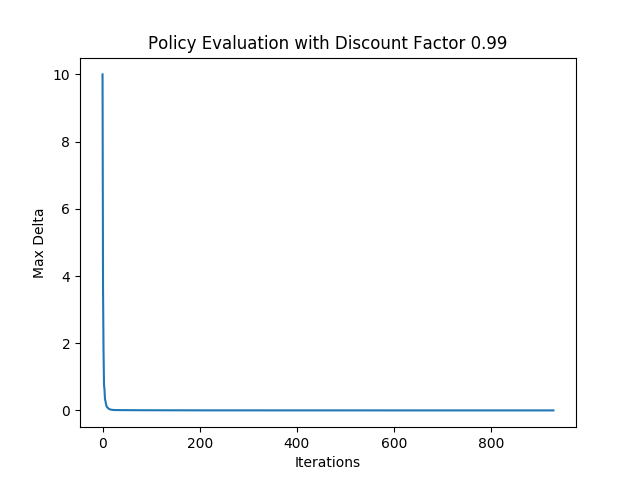
\includegraphics[scale=0.7]{policy_evaluation_99}
\centering
\caption{Convergence of policy evaluation}
\end{figure}


% VALUE ITERATION---------------------------------------------------------------
\newpage
\section{Value Iteration}
\textbf{In a separate file called value\_iteration.py, provide a complete
implementation of the value iteration.}
\\

\noindent
\textbf{-}
\noindent
\textbf{Did your algorithm converge at all?}
\\

\noindent
In this work, the value iteration algorithm was used to find the optimal policy
at 3 different discount factors; namely, 0.8, 0.95 and 0.99. In our case, the
value iteration algorithm converged at all discount factors with a threshold of
$10^{-6}$ as described in the problem.\\


\noindent
\textbf{-}
\noindent
\textbf{How many iterations did this take for each value of $\gamma$ ?}
\\

\noindent
As seen in figure 4, different discount factors resulted in different numbers of
total iterations necessary to converge. In our case, a discount factor of 0.8,
0.95 and 0.99 have a total iterations of 74, 316, and 1605, respectively. In the
left column, the convergence graph shows that the max delta decreases
exponentially over the aforementioned interations to a value that is ultimately
within the acceptable threshold.
\\

\noindent
\textbf{-}
\noindent
\textbf{What is the best value of $\gamma$? Also, What was the final policy you
obtained for each value of $\gamma$?}
\\

\noindent
In terms of iterations, the best discount factor is 0.8 as it converged the
fastest. In terms of policy that favors long term rewards, 0.95 is better than
0.99 as both achieved the same optimal policy while 0.95 took only 20\% of the
time it took 0.99 to converge. While the policy is the same in most states, the
main difference between the optimal policy with 0.8 discount factor and
0.95/0.99 discount factor are states (1,3) and (1,4). In discount factor 0.8,
the policy outputs "up" in these states because it is favoring short term
rewards by reaching state B (0,3) for a +5 reward. Conversely, the agent favors
long term rewards for discount factor 0.95/0.99; therefore, the policy outputs
"left" in the aforementioned states, helping the agent to skip state B and reach
state A. The full policy for each discount factor can be seen in figure 4.
\\

\noindent
\textbf{-}
\noindent
\textbf{Does the optimal policy you obtained correspond to the policy you
conjectured earlier?}
\\

\noindent
Yes, it does.
\\

\newpage
\begin{figure}[h]
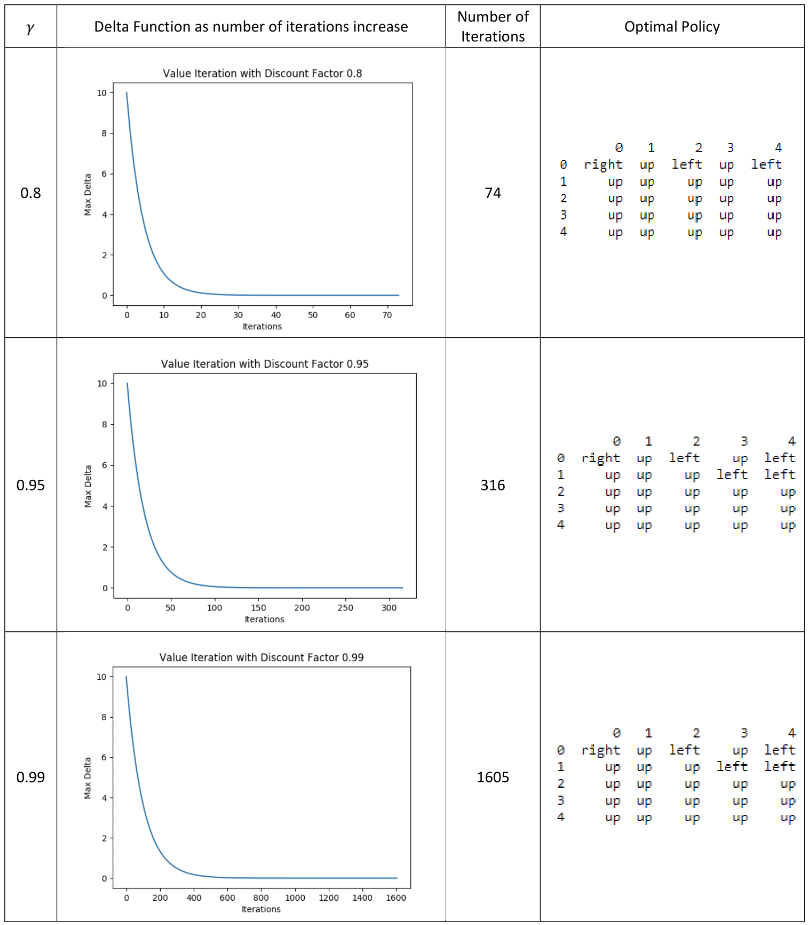
\includegraphics[scale=0.5]{VI_chart}
\centering
\caption{Value iteration results: convergence graph, total iterations, optimal policy}
\end{figure}


% POLICY ITERATION---------------------------------------------------------------
\newpage
\section{Policy Iteration}
\textbf{Implement the policy iteration algorithm in a file called
policy\_iteration.py.}
\\

\noindent
\textbf{-}
\noindent
\textbf{Did your algorithm converge at all?}
\\

\noindent
Similar to value iteration, policy iteration was implemented in this work and
tested with the same 3 discount factors, 0.8, 0.95 and 0.99. In our case, all
three discount factors converged. The convergence graph is seen in the left
column of figure 5. Because policy iteration consists of 2 steps: policy
evaluation and policy improvement, the evaluation part first converges on a
value function and then the improvement step extracts a policy from the value
function. The algorithm then takes this policy to create a new value function
that is then used to extract a new policy. This process repeats until the policy
becomes stable. Because of this two step process. the convergence graph shows
different spikes which represents the iteration where a new policy is being
evaluated.
\\

\noindent
\textbf{-}
\noindent
\textbf{How many iterations did this take for each value of $\gamma$ ?}
\\

\noindent
Different discount factor values led to different numbers of iterations for
convergence. As seen in figure 5, discount factors of 0.8, 0.95 and 0.99 have
total iterations of 192, 1447 and 7349, respectively. It is also worth noting
that the policy often converges faster than the values as shown in the brackets
in the second column of figure 5. In this case, the policy converged in 118,
1131 and 5744 iterations for discount factors of 0.8, 0.95 and 0.99
respectively. \\

\noindent
\textbf{-}
\noindent
\textbf{What is the best value of $\gamma$? Also, What was the final policy you
obtained for each value of $\gamma$?}
\\

\noindent
Similar to value iteration, the best discount factor value in terms of number of
iterations is 0.8 as it converged the fastest. In terms of favoring future
rewards, similar behaviour to value iteration is seen here as well where 0.95
converged much faster than 0.99 while the final optimal policy between the two
remain identical. The final optimal policy for each discount factor is presented
in figure 5. \\

\noindent
\textbf{-}
\noindent
\textbf{Does the optimal policy you obtained correspond to the policy you
conjectured earlier?}
\\

\noindent
Yes, it does.
\\

\newpage
\begin{figure}[h]
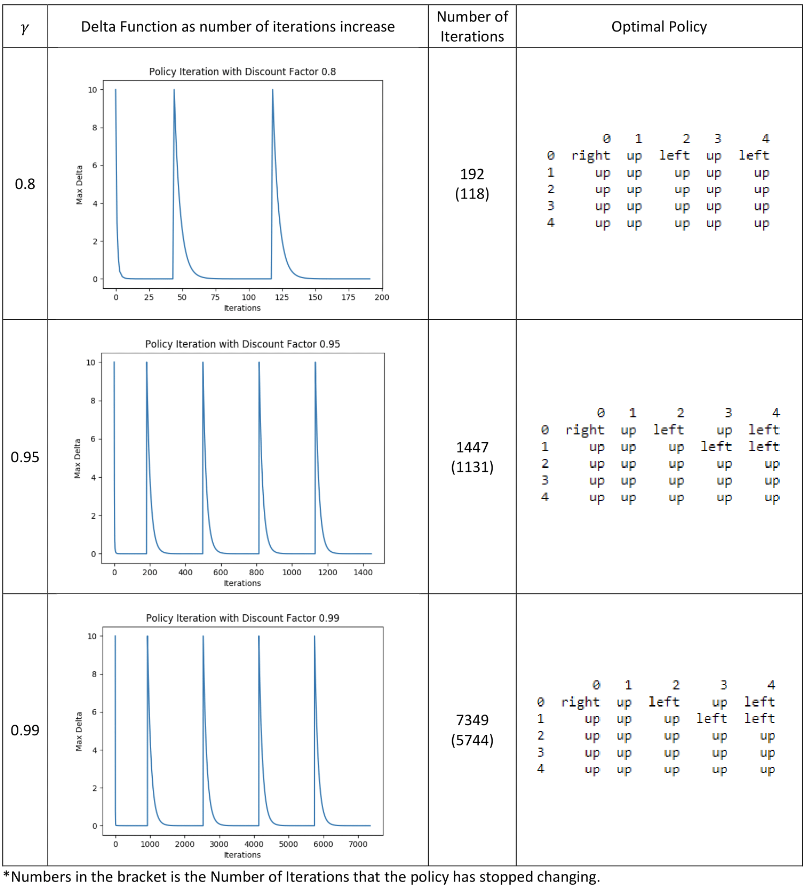
\includegraphics[scale=0.5]{PI_chart}
\centering
\caption{Policy iteration results: convergence graph, total iterations, optimal policy}
\end{figure}


% ALGORITHM COMPARISON---------------------------------------------------------------
\newpage
\section{Comparison of Algorithms}
\textbf{In the final section of your report, you must compare the two algorithms you
implemented and their performance on the Gridworld domain, and comment on any
differences you observed. In particular, please answer at least the following
questions in your report:}
\\

\noindent
The following shows a table of the different value functions achieved with each algorithm at 
3 different discount factors.\\

\begin{figure}[h]
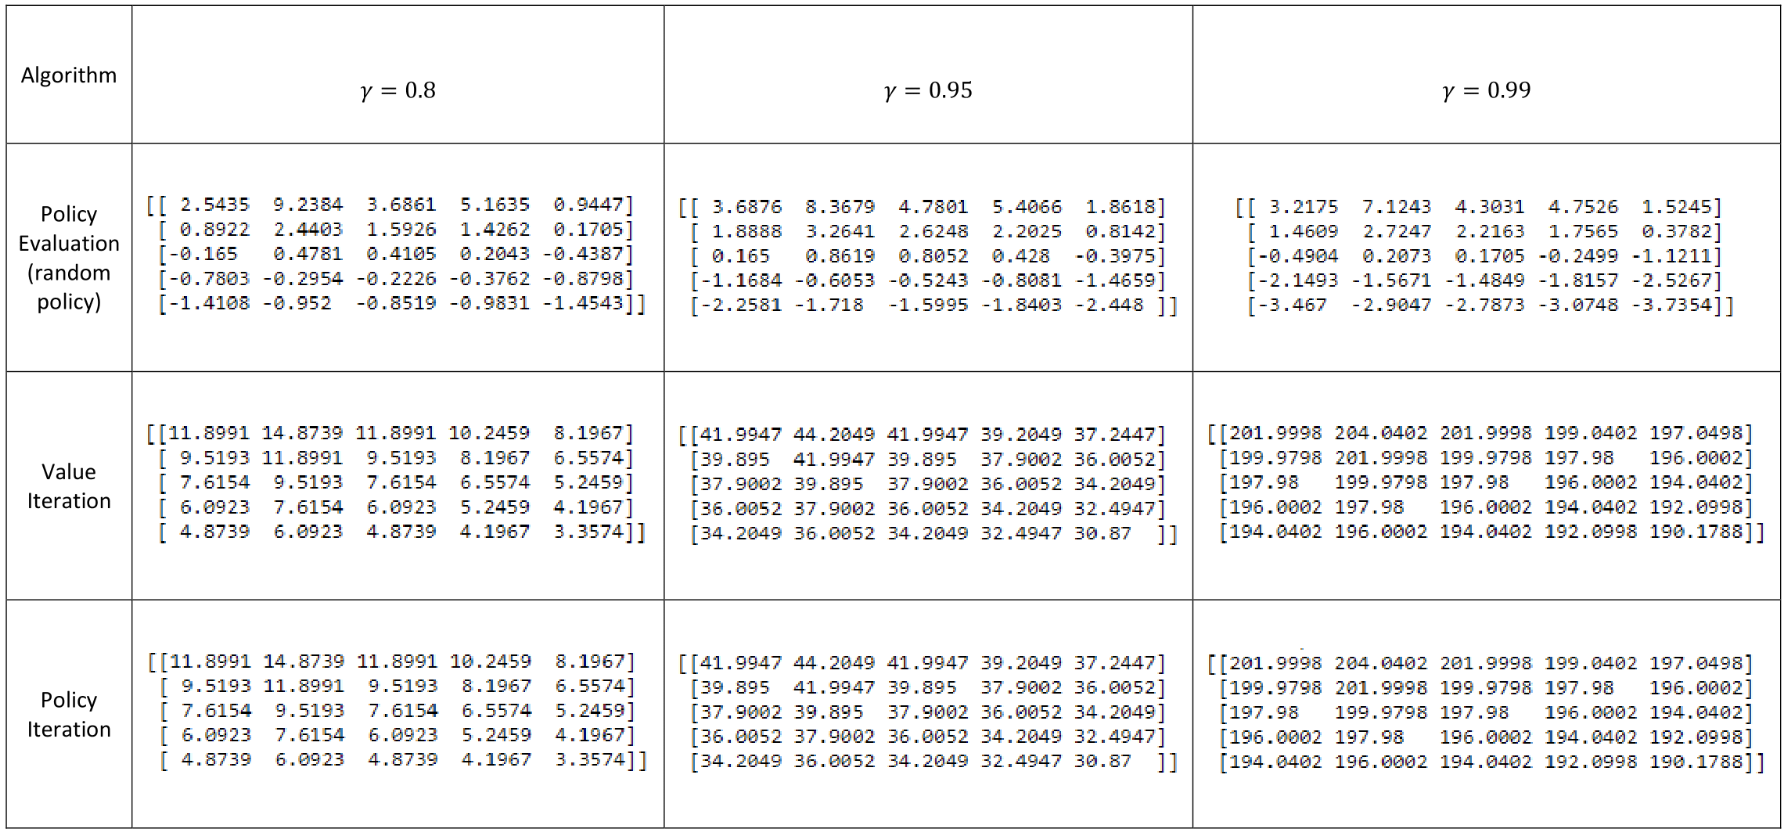
\includegraphics[scale=0.255]{value_functions}
\centering
\caption{Value functions of policy evaluation, value iteration and policy iteration}
\end{figure}

\noindent
\textbf{-}
\noindent
\textbf{Compare the performance (e.g. values) of the optimal policies obtained
using value and policy iteration to the performance of the policy that chooses
an action at random (as you analyzed earlier), and comment on the difference.}
\\

\noindent
The value functions obtained from both algorithms are identical for each state
across all discount factors as seen in figure 6. Both algorithms provide larger
values than the random policy evaluation (figure 2), and the difference
increases as discount factor increases. Even if the random policy were the
optimal policy, the state value will always be lower in policy evaluation
because there is no improvement step. This is because state values won’t
increase as they are being updated, which causes its performance to be inferior
to the iterative methods. \\

\noindent
\textbf{-}
\noindent
\textbf{Were the value functions and policies you obtained, and the number of
iterations required to obtain these policies, similar between algorithms? How do
your results differ for different values of the parameter(s) (e.g. $\gamma$)?}
\\

\noindent
We obtained the same value functions and policies from both value and policy
iteration. Our results showed that value iteration required less number of
iterations than policy iteration. For example, when discount factor is 0.99, the
number of iterations of policy iteration is 7349 and value iteration is 1605;
when discount factor is 0.95, the number of iterations of policy iteration is
1447 and value iteration is 316; when discount factor is 0.80, the number of
iterations of Policy iteration is 192 and Value Iteration is 74.\\

\noindent
The extra iteration count during policy iteration is due to policy evaluation.
Each policy evaluation starts with the value function obtained with the previous
policy. As shown in the delta function graphs in figure 5, the iterations
between two local max deltas represent the policy evaluation steps where the
algorithm tries to converge on the value function while the local max delta
appears when there is a new policy. Since the initial policy is randomly
generated, we tried different runs and we found that starting from different
initial policy will change the total number of iteration, but it won’t change
the optimal states values and the optimal policy. \\

\noindent
Value iterations have less number of iterations because the algorithm truncates
policy evaluation. The designed algorithm updates all values of cells based on
the previous value functions, and progressively the value function converges.
Once optimal value functions are found for all cells, one sweep of policy
improvement with greedy search is performed to find the optimal policy. \\

\noindent
\textbf{-}
\noindent
\textbf{Which algorithm was more difficult to implement and why? Which algorithm
do you think would work better if the problem was scaled up?}
\\

\noindent
Between policy and value iteration, policy iteration was more difficult to
implement because it required more steps (policy evaluation and improvement).
More specifically, the policy evaluation must first sweeps through every state
to converge on a value for each state and then the improvement algorithm must
sweep through every state to find the best action to take in each state.\\

\noindent
We evaluated the number of iterations for both algorithms, value iterations has
shown less iterations for each different discount factor, yet policy iteration
found the optimal policy before the value converges (for =0.99, optimal policy
was found 1605 iterations before value converges); therefore, if the problem was
scaled up, policy iterations would work better since it will always converge to
the optimal policy. \\

\noindent
\textbf{-}
\noindent
\textbf{Include any additional insights, challenges, or important observations
that you discovered while building or running your experiments.}
\\

\noindent
Challenge 1: It was found that there are two ways to update cells(states). First
way is to update the cell with its new found value, and computation of values of
the following cells is based on the new value. Second way is to update all the
cells at the end, and they are updated all at once. The difference is whether
you update the cells inside the for loop or outside the for loop. \\

\noindent
For policy iteration, both ways will lead to convergence. The second way will
take more iterations than the first way. \\

\noindent
For value iteration, the first way will not converge, and the second way will
converge.  In the first way, we initiate cells value with 0, and we get new
cells value with only A being 10, B being 5 and the rest of them being 0 . This
leads delta for some cells to be 0, which is less the threshold set ($10^{-6}$),
then breaks the loop without maximizing the policy evaluation update. \\

\noindent
In addition, one of the main challenges for the implementation of both algorithms
has been the full backup of certains values. The iterative nature of the
operations in the code requires backup for states values as we are estimating
new values for each possible next state. For the implementation of value
titeration, we tried to update the values for each state as soon as new
calculations are available, yet it didn’t converge because it entered in a loop
of value updating and some values were not better than the old. Policy iteration
needs to back up more values than Value Iteration, so the main challenge was to
ensure that every state value and policy has a full backup before a new
iteration and don’t update old value until they are compared with new results
and calculate its convergence rate (delta). \\

% APPENDIX-------------------------------------
\newpage
\section{Appendix}

\begin{figure}[h]
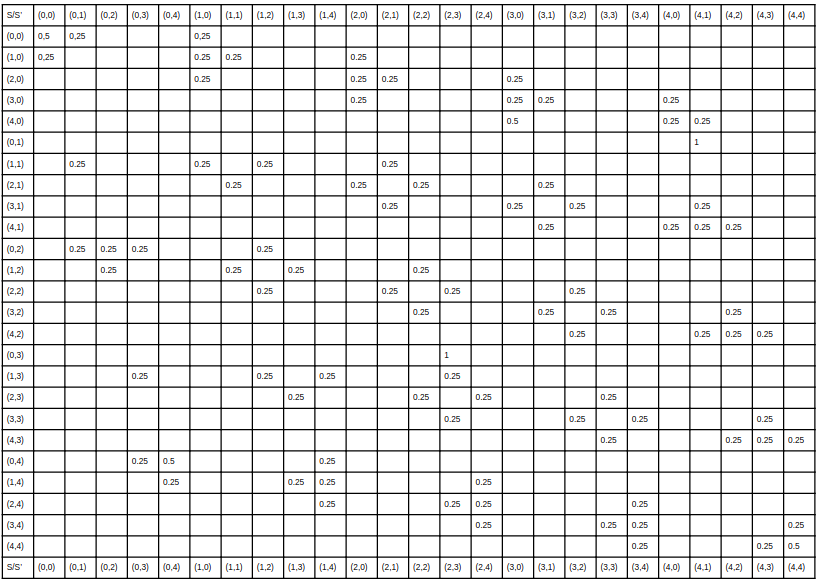
\includegraphics[scale=0.5]{transition_matrix}
\centering
\caption{Transition Matrix}
\end{figure}

\end{document}
